\documentclass{beamer}

\usepackage{graphicx}
\usepackage{booktabs}\title[Chiselizing SDR Blocks]{Chiselizing SDR Blocks}
\author{Albert Magyar}
\date{\today}

\begin{document}
\begin{frame}
\titlepage
\end{frame}

\begin{frame}
\frametitle{Overview}
\begin{itemize}
\item Intro to RFNoC
\item RFNoC Blocks
\item Example: \texttt{addsub}
\item Recurring patterns in Verilog and Chisel
\item Goals
\end{itemize}
\end{frame}

\begin{frame}
\frametitle{Intro to RFNoC}
\begin{center}
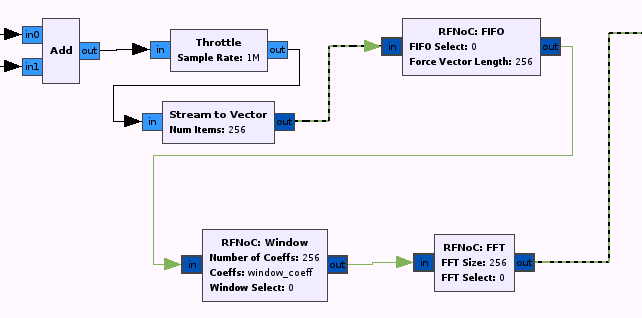
\includegraphics[width=3.5in]{images/gnu_radio_rfnoc.png}
\end{center}
\begin{itemize}
\item FPGA toolkit for GNU radio
\item Allows chaining of hardware and software blocks 
\end{itemize}
\end{frame}

\begin{frame}
\frametitle{Intro to RFNoC}
\begin{itemize}
\item Accelerators implemented in Verilog
\item NoC: packet headers on top of AXI4 Streaming crossbar
\item Designers write parametrized blocks with ready/valid/last and settings registers
\end{itemize}
\end{frame}

\begin{frame}
\frametitle{Intro to RFNoC}
\begin{itemize}
\item Designers write parametrized blocks
\item GNU Radio frontend elaborates instances
\item RFNoC configurator assigns endpoint addresses and parametrizes RFNoC shim modules (\texttt{noc\_shell}) 
\item Parametrizes and generates Verilog for NoC
\end{itemize}
\end{frame}

\begin{frame}
\frametitle{RFNoC Blocks}
\begin{itemize}
\item Simple, fixed-function DSP blocks
\item Blocks have simple FIFO interfaces
\item Export parameters to the GNU Radio space
\item Identity as RFNoC endpoint transparent to designer
\item<2-> \emph{We want people to write these in Chisel}
\end{itemize}
\end{frame}

\begin{frame}
\frametitle{Example: \texttt{addsub}}
\begin{center}
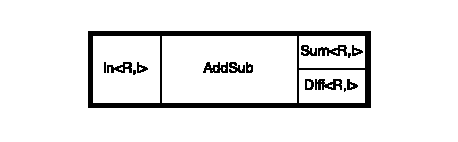
\includegraphics[width=2.5in]{figs/addsub.pdf}
\end{center}
\begin{itemize}
\item Simple variable-width complex adder/subtractor
\item FIFO inputs
\end{itemize}
\end{frame}

\begin{frame}
\frametitle{Patterns: splitting FIFOs}
\begin{center}
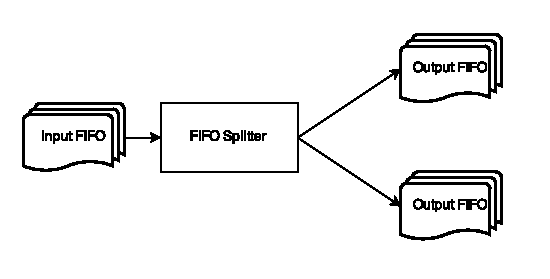
\includegraphics[width=2.5in]{figs/fifo_splitter.pdf}
\end{center}
\begin{itemize}
\item Hard to do right
\item Don't let ready depend on valid
\end{itemize}
\end{frame}

\begin{frame}[fragile]
\frametitle{Verilog}
\tiny
\begin{verbatim}
generate
if(ACTIVE_MASK[0])
	axi_fifo_short #(.WIDTH(WIDTH+1)) short_fifo0
	  (.clk(clk), .reset(reset), .clear(clear),
	   .i_tdata({o0_tlast_int, o0_tdata_int}), .i_tvalid(o0_tvalid_int), .i_tready(o0_tready_int),
	   .o_tdata({o0_tlast, o0_tdata}), .o_tvalid(o0_tvalid), .o_tready(o0_tready));
if(ACTIVE_MASK[1])
	axi_fifo_short #(.WIDTH(WIDTH+1)) short_fifo1
	  (.clk(clk), .reset(reset), .clear(clear),
	   .i_tdata({o1_tlast_int, o1_tdata_int}), .i_tvalid(o1_tvalid_int), .i_tready(o1_tready_int),
	   .o_tdata({o1_tlast, o1_tdata}), .o_tvalid(o1_tvalid), .o_tready(o1_tready));
if(ACTIVE_MASK[2])
	axi_fifo_short #(.WIDTH(WIDTH+1)) short_fifo2
	  (.clk(clk), .reset(reset), .clear(clear),
	   .i_tdata({o2_tlast_int, o2_tdata_int}), .i_tvalid(o2_tvalid_int), .i_tready(o2_tready_int),
	   .o_tdata({o2_tlast, o2_tdata}), .o_tvalid(o2_tvalid), .o_tready(o2_tready));
if(ACTIVE_MASK[3])
	axi_fifo_short #(.WIDTH(WIDTH+1)) short_fifo3
	  (.clk(clk), .reset(reset), .clear(clear),
	   .i_tdata({o3_tlast_int, o3_tdata_int}), .i_tvalid(o3_tvalid_int), .i_tready(o3_tready_int),
	      .o_tdata({o3_tlast, o3_tdata}), .o_tvalid(o3_tvalid), .o_tready(o3_tready));
endgenerate
\end{verbatim}
\end{frame}

\begin{frame}
\frametitle{Problems}
\begin{itemize}
\item Classic generate block
\item No indirection of signals
\end{itemize}
\end{frame}


\begin{frame}[fragile]
\frametitle{Module-level reuse}
\tiny
\begin{verbatim}
module split_stream_fifo
  #(parameter WIDTH=16,
    parameter ACTIVE_MASK=4'b1111)
   (input clk, input reset, input clear,
    input [WIDTH-1:0] i_tdata, input i_tlast, input i_tvalid, output i_tready,
    output [WIDTH-1:0] o0_tdata, output o0_tlast, output o0_tvalid, input o0_tready,
    output [WIDTH-1:0] o1_tdata, output o1_tlast, output o1_tvalid, input o1_tready,
    output [WIDTH-1:0] o2_tdata, output o2_tlast, output o2_tvalid, input o2_tready,
    output [WIDTH-1:0] o3_tdata, output o3_tlast, output o3_tvalid, input o3_tready);
\end{verbatim}
\end{frame}

\begin{frame}
\frametitle{Problems}
\begin{itemize}
\item Module-level reuse seems nice
\item Does it make sense for hardware?
\item<2-> RTL designers want to reuse implementations
\item<2-> RTL-level designs are tightly coupled
\item<2-> Interface-level inheritance often gets in the way
\end{itemize}
\end{frame}

\begin{frame}[fragile]
\frametitle{Module-level reuse}
\tiny
\begin{verbatim}
module split_stream_fifo
  #(parameter WIDTH=16,
    parameter ACTIVE_MASK=4'b1111)
   (input clk, input reset, input clear,
    input [WIDTH-1:0] i_tdata, input i_tlast, input i_tvalid, output i_tready,
    output [WIDTH-1:0] o0_tdata, output o0_tlast, output o0_tvalid, input o0_tready,
    output [WIDTH-1:0] o1_tdata, output o1_tlast, output o1_tvalid, input o1_tready,
    output [WIDTH-1:0] o2_tdata, output o2_tlast, output o2_tvalid, input o2_tready,
    output [WIDTH-1:0] o3_tdata, output o3_tlast, output o3_tvalid, input o3_tready);
\end{verbatim}
\textbf{Compounded by fixed portlists in Verilog!}
\end{frame}

\begin{frame}[fragile]
\frametitle{Chisel: flexible implementation reuse}
\tiny
\begin{verbatim}
object SplitDecoupled {
  def apply[T <: Data](in: DecoupledIO[T], n: Int): Seq[DecoupledIO[T]] = {
    val outs = Seq.fill(n){ in.clone }
    var iready = Bool(true)
    for (i <- 0 until n) {
      iready = iready && outs(i).ready
      var ovalid = in.valid
      for (j <- 0 until n) {
        if (i != j) ovalid = ovalid && outs(j).ready
      }
      outs(i).valid := ovalid
      outs(i).bits := in.bits
    }
    in.ready := iready
    outs
  }
}
\end{verbatim}
\end{frame}


\end{document}